\documentclass[10pt]{ltjsarticle}
\usepackage{booktabs}
\usepackage{graphicx}
\usepackage{amsmath, amssymb}
\usepackage{multirow}
\usepackage{url}
\usepackage{listings} 

\begin{document}

\title{4.How to improve detecting AI voice changer with HuBERT 
\\HuBERTを用いたボイスチェンジャ検出の改良}
\author{柴沼 厳 Itsuki Shibanuma     蓬莱 尚幸 Hisayuki Horai}

\maketitle

\section{はじめに}

音声のディープフェイクを利用した詐欺、ビデオ会議でのディープフェイクを利用した詐欺、政治家を装ったディープフェイクによる情報操作など近年、ディープフェイク技術を利用した悪用が増加している。音声のディープフェイク技術は、小さなデータセットで、特定の人物の声を再現し相手を騙すことができるため、特に危険である。本研究では、RVCと呼ばれる音声変換技術を用いたAIボイスチェンジャーの検出における改善手法を提案する。RVC(Retrieval-Based Voice Conversion)は、リアルタイムでの音声変換(VC: Voice Conversion)が可能なAIボイスチェンジャーであり、内部でHuBERTというモデルを使用している。本研究における提案手法は、HuBERTを用いたAIボイスチェンジャーの検出手法であり、HuBERTの最終出力層に、CNNを用いた特徴量を加えることで安定した検出を実現する。

\section{HuBERTのモデル構造と数式の詳細解説}

\subsection{モデル構造の概要}
HuBERTは、音声データの高精度な表現学習を目的としており、以下の2つの主要なステップを特徴とする:
\begin{enumerate}
    \item \textbf{クラスタリングを用いた目標生成}:
    音声データを事前にクラスタリングし、離散的な「隠れ単位」(hidden units) を生成します。例えば、K-meansクラスタリングを用いて音声データを100または500クラスに分類します。
    \item \textbf{マスクされた予測 (Masked Prediction)}:
    マスクされた入力音声データを使用し、マスクされた部分の隠れ単位を予測するタスクを学習します。これにより、非マスク領域の情報を基にマスク領域を推測する能力がモデルに学習されます。
\end{enumerate}

HuBERTは、BERTアーキテクチャを応用し、音声データの時間的構造と高次元表現の両方を学習する。
\cite{HuBERT}.

\subsection{数式の詳細}

\subsubsection{クラスタリングを用いた隠れ単位の生成}
HuBERTでは、音声データ \( X \) を \( T \) フレームの系列として表現する:
\[
X = [x_1, x_2, \dots, x_T]
\]
クラスタリングモデル \( h \) を使用して、各フレーム \( x_t \) にクラスタラベル \( z_t \) を割り当てる:
\[
Z = h(X) = [z_1, z_2, \dots, z_T], \quad z_t \in \{1, \dots, C\}
\]
ここで、\( C \) はクラスタ数である(例:\( C = 100 \))。

\subsubsection{マスクされた予測の学習}
HuBERTは、以下のようにマスクされた音声データ \( \tilde{X} \) を生成する:
\[
\tilde{X} = r(X, M)
\]
ここで、\( M \subseteq \{1, \dots, T\} \) はマスクされたフレームのインデックス集合、\( r(\cdot) \) は対応するフレームをマスク埋め込み \( \tilde{x} \) に置き換える操作を表す。

モデル \( f \) は、マスクされたデータ \( \tilde{X} \) を入力とし、各タイムステップ \( t \) の目標分布を予測する:
\[
p_f(z_t | \tilde{X}, t)
\]

\subsubsection{損失関数}
HuBERTの損失関数は、マスクされた領域 \( M \) と非マスク領域に基づくクロスエントロピー損失の重み付き和として定義される:
\[
L = \alpha L_m + (1 - \alpha) L_u
\]
\begin{itemize}
    \item マスクされた領域での損失:
    \[
    L_m(f; X, M, Z) = -\sum_{t \in M} \log p_f(z_t | \tilde{X}, t)
    \]
    \item 非マスク領域での損失:
    \[
    L_u(f; X, M, Z) = -\sum_{t \notin M} \log p_f(z_t | \tilde{X}, t)
    \]
\end{itemize}
ここで、\( \alpha \) は損失関数の重みを調整するハイパーパラメータである。特に、\( \alpha = 1 \) の場合、損失はマスク領域のみに基づく。

\subsection{モデル構成}
HuBERTモデルは以下の構成を持つ:
\begin{enumerate}
    \item \textbf{畳み込みエンコーダ}:
    音声波形を低次元表現に変換する。
    \item \textbf{BERTエンコーダ}:
    Transformerアーキテクチャを用いて、時間的相関をモデル化する。
    \item \textbf{射影層}:
    特徴量をクラスタリングラベルの分布に変換する。
\end{enumerate}

\begin{figure}
\centering
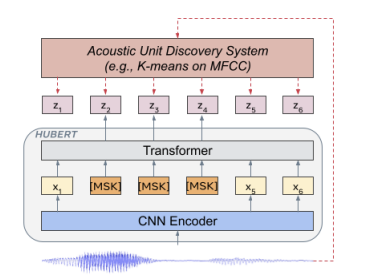
\includegraphics[width=70mm]{./img/HuBERT.png} 
\caption{{図 1}: HuBERTアプローチは、k-meansクラスタリングを1回または複数回繰り返すことで生成されたマスクされたフレーム(図中の \( y_2, y_3, y_4 \))の隠れクラスタ割り当てを予測する。}
\end{figure}


\section{提案手法}

従来手法である、音声データから得られたMFCCをCNNによって分類するモデルでは、90\%以上の精度を達成を達成することはできないが、とても学習コストが低く、ロバストな学習が可能であった。一方、HuBERTを単体で用いたモデルでは、学習コストが高く、ロバストな学習が難しいが、90\%以上の精度を達成することができる。そこで、HuBERTの高い精度とCNNのロバスト性を組み合わせることで、安定した学習と高い精度を両立することができると考えた。

今回私が提案する手法は以下のとおりである。

まず初めに、音声データから得られたMFCCをCNNによって、(1,768)のテンソルに変換する。そうして得られたテンソルをHuBERTの最終出力層と足し合わせる。

次に、このテンソルをLinear層に入力し、最終的にSoftmax関数によって2クラス分類を行う。このような構成を取ることで、HuBERTの高い精度とCNNのロバスト性を組み合わせることができる。

\section{実験}

\subsection{実験設定}

RVCを用いて変換された音声データを500、未変換の音声データを500、計1000のデータセットを作成した。その中から、ランダムサンプリングにより、訓練データとテストデータをそれぞれ400、100のデータセットを作成し、実験を行った。実験で使用したモデルは、従来手法である、音声データから得られたMFCCをCNNによって分類するモデル、HuBERTを単体で用いたモデル、提案手法であるHuBERTとCNNを組み合わせたモデルの計3つである。これらのモデルに対して、入力された音声がRVCを用いて変換されたものか、そうでないかの2クラス分類を行うように学習した。

今回の実験において、HuBERTを単体で用いたモデルと、HuBERTとCNNを組み合わせたモデルの学習において、モデルのロバスト性を確認するため、エポック数を10、20という比較的大きな値に設定した。
\subsection{モデル構成}

CNNを用いたモデルの構成は以下の通りである。
\begin{lstlisting}[language=Python]
CNNClassifier(
    (conv1): Conv2d(1, 16, kernel_size=(3, 3), stride=(1, 1), padding=(1, 1))
    (bn1): BatchNorm2d(16, eps=1e-05, momentum=0.1, affine=True, track_running_stats=True)
    (conv2): Conv2d(16, 32, kernel_size=(3, 3), stride=(1, 1), padding=(1, 1))
    (bn2): BatchNorm2d(32, eps=1e-05, momentum=0.1, affine=True, track_running_stats=True)
    (pool): MaxPool2d(kernel_size=2, stride=2, padding=0, dilation=1, ceil_mode=False)
    (dropout_conv): Dropout(p=0.3, inplace=False)
    (fc1): Linear(in_features=10240, out_features=128, bias=True)
    (dropout_fc): Dropout(p=0.5, inplace=False)
    (fc2): Linear(in_features=128, out_features=2, bias=True)
)
\end{lstlisting}

HuBERTを単体で用いたモデルの構成は以下の通りである。

\begin{lstlisting}[language=Python]
HubertForSequenceClassification(
  (hubert): HubertModel(
    (feature_extractor): HubertFeatureEncoder(
      (conv_layers): ModuleList(
        (0): HubertGroupNormConvLayer(
          (conv): Conv1d(1, 512, kernel_size=(10,), stride=(5,), bias=False)
          (activation): GELUActivation()
          (layer_norm): GroupNorm(512, 512, eps=1e-05, affine=True)
        )
        (1-4): 4 x HubertNoLayerNormConvLayer(
          (conv): Conv1d(512, 512, kernel_size=(3,), stride=(2,), bias=False)
          (activation): GELUActivation()
        )
        (5-6): 2 x HubertNoLayerNormConvLayer(
          (conv): Conv1d(512, 512, kernel_size=(2,), stride=(2,), bias=False)
          (activation): GELUActivation()
        )
      )
    )
    (feature_projection): HubertFeatureProjection(
      (layer_norm): LayerNorm((512,), eps=1e-05, elementwise_affine=True)
      (projection): Linear(in_features=512, out_features=768, bias=True)
      (dropout): Dropout(p=0.0, inplace=False)
    )
    (encoder): HubertEncoder(
      (pos_conv_embed): HubertPositionalConvEmbedding(
        (conv): ParametrizedConv1d(
          768, 768, kernel_size=(128,), stride=(1,), padding=(64,), groups=16
          (parametrizations): ModuleDict(
            (weight): ParametrizationList(
              (0): _WeightNorm()
            )
          )
        )
        (padding): HubertSamePadLayer()
        (activation): GELUActivation()
      )
      (layer_norm): LayerNorm((768,), eps=1e-05, elementwise_affine=True)
      (dropout): Dropout(p=0.1, inplace=False)
      (layers): ModuleList(
        (0-11): 12 x HubertEncoderLayer(
          (attention): HubertSdpaAttention(
            (k_proj): Linear(in_features=768, out_features=768, bias=True)
            (v_proj): Linear(in_features=768, out_features=768, bias=True)
            (q_proj): Linear(in_features=768, out_features=768, bias=True)
            (out_proj): Linear(in_features=768, out_features=768, bias=True)
          )
          (dropout): Dropout(p=0.1, inplace=False)
          (layer_norm): LayerNorm((768,), eps=1e-05, elementwise_affine=True)
          (feed_forward): HubertFeedForward(
            (intermediate_dropout): Dropout(p=0.1, inplace=False)
            (intermediate_dense): Linear(in_features=768, out_features=3072, bias=True)
            (intermediate_act_fn): GELUActivation()
            (output_dense): Linear(in_features=3072, out_features=768, bias=True)
            (output_dropout): Dropout(p=0.1, inplace=False)
          )
          (final_layer_norm): LayerNorm((768,), eps=1e-05, elementwise_affine=True)
        )
      )
    )
  )
  (projector): Linear(in_features=768, out_features=256, bias=True)
  (classifier): Linear(in_features=256, out_features=2, bias=True)
)
\end{lstlisting}

HuBERTとCNNを組み合わせたモデルの構成は以下の通りである。

\begin{lstlisting}[language=Python]
HuBERTWithLogMel(
    (hubert): HubertModel(
        (feature_extractor): HubertFeatureEncoder(
            (conv_layers): ModuleList(
                (0): HubertGroupNormConvLayer(
                    (conv): Conv1d(1, 512, kernel_size=(10,), stride=(5,), bias=False)
                    (activation): GELUActivation()
                    (layer_norm): GroupNorm(512, 512, eps=1e-05, affine=True)
                )
                (1-4): 4 x HubertNoLayerNormConvLayer(
                    (conv): Conv1d(512, 512, kernel_size=(3,), stride=(2,), bias=False)
                    (activation): GELUActivation()
                )
                (5-6): 2 x HubertNoLayerNormConvLayer(
                    (conv): Conv1d(512, 512, kernel_size=(2,), stride=(2,), bias=False)
                    (activation): GELUActivation()
                )
            )
        )
        (feature_projection): HubertFeatureProjection(
            (layer_norm): LayerNorm((512,), eps=1e-05, elementwise_affine=True)
            (projection): Linear(in_features=512, out_features=768, bias=True)
            (dropout): Dropout(p=0.0, inplace=False)
        )
        (encoder): HubertEncoder(
            (pos_conv_embed): HubertPositionalConvEmbedding(
                (conv): ParametrizedConv1d(
                    768, 768, kernel_size=(128,), stride=(1,),
                    padding=(64,), groups=16
                    (parametrizations): ModuleDict(
                        (weight): ParametrizationList(
                            (0): _WeightNorm()
                        )
                    )
                )
                (padding): HubertSamePadLayer()
                (activation): GELUActivation()
            )
            (layer_norm): LayerNorm((768,), eps=1e-05, elementwise_affine=True)
            (dropout): Dropout(p=0.1, inplace=False)
            (layers): ModuleList(
                (0-11): 12 x HubertEncoderLayer(
                    (attention): HubertSdpaAttention(
                        (k_proj): Linear(in_features=768, out_features=768, bias=True)
                        (v_proj): Linear(in_features=768, out_features=768, bias=True)
                        (q_proj): Linear(in_features=768, out_features=768, bias=True)
                        (out_proj): Linear(in_features=768, out_features=768, bias=True)
                    )
                    (dropout): Dropout(p=0.1, inplace=False)
                    (layer_norm): LayerNorm((768,), eps=1e-05, elementwise_affine=True)
                    (feed_forward): HubertFeedForward(
                        (intermediate_dropout): Dropout(p=0.1, inplace=False)
                        (intermediate_dense): Linear(in_features=768, out_features=3072, bias=True)
                        (intermediate_act_fn): GELUActivation()
                        (output_dense): Linear(in_features=3072, out_features=768, bias=True)
                        (output_dropout): Dropout(p=0.1, inplace=False)
                    )
                    (final_layer_norm): LayerNorm((768,), eps=1e-05, elementwise_affine=True)
                )
            )
        )
    )
    (cnn): Sequential(
        (0): Conv2d(1, 32, kernel_size=(3, 3), stride=(1, 1), padding=(1, 1))
        (1): ReLU()
        (2): MaxPool2d(kernel_size=2, stride=2, padding=0, dilation=1, ceil_mode=False)
        (3): Conv2d(32, 64, kernel_size=(3, 3), stride=(1, 1), padding=(1, 1))
        (4): ReLU()
        (5): MaxPool2d(kernel_size=2, stride=2, padding=0, dilation=1, ceil_mode=False)
    )
    (fc_mel): Linear(in_features=1228800, out_features=768, bias=True)
    (classifier): Linear(in_features=768, out_features=2, bias=True)
    (loss_fn): CrossEntropyLoss()
)
\end{lstlisting}

\subsection{結果}

CNNを用いたモデルによる推論結果は表1の通りである。
\vspace{5pt}
\begin{table}[h]
\centering
\caption{CNNを用いたモデルによる推論結果(epoch=10)}
\begin{tabular}{cccc}
\toprule
Epoch & Training Loss & Validation Loss & Accuracy (\%) \\
\midrule
1 & 0.3538 & 0.2456 & 84.00 \\
2 & 0.1742 & 0.2422 & 88.00 \\
3 & 0.1368 & 0.2535 & 80.00 \\
4 & 0.1663 & 0.2592 & 80.00 \\
5 & 0.1886 & 0.2644 & 80.00 \\
6 & 0.1164 & 0.2791 & 80.00 \\
7 & 0.1543 & 0.2832 & 80.00 \\
8 & 0.2481 & 0.2811 & 80.00 \\
9 & 0.1784 & 0.2664 & 80.00 \\
10 & 0.1607 & 0.2556 & 80.00 \\
\bottomrule
\end{tabular}
\end{table}


また、HuBERTを単体で用いたモデルによる推論結果は表2、表3の通りである。
\vspace{10pt}
\begin{table}[h]
\centering
\caption{HuBERTを単体で用いたモデルによる推論結果(epoch=10)}
\begin{tabular}{cccc}
\toprule
Epoch & Training Loss & Validation Loss & Accuracy (\%) \\
\midrule
1  & 0.698800 & 0.695777 & 50.00 \\
2  & 0.694900 & 0.694842 & 50.00 \\
3  & 0.696400 & 0.693102 & 50.00 \\
4  & 0.690300 & 0.688122 & 50.00 \\
5  & 0.681000 & 0.665364 & 100.00 \\
6  & 0.657100 & 0.606551 & 100.00 \\
7  & 0.549300 & 0.524111 & 93.75 \\
8  & 0.489800 & 0.403892 & 93.75 \\
9  & 0.366900 & 0.325082 & 93.75 \\
10 & 0.262000 & 0.198047 & 100.00 \\
\bottomrule
\end{tabular}
\end{table}


\begin{table}[h]
\centering
\caption{HuBERTを単体で用いたモデルによる推論結果(epoch=20)}
\begin{tabular}{c c c c}
\hline
\textbf{Epoch} & \textbf{Training Loss} & \textbf{Validation Loss} & \textbf{Accuracy} \\
\hline
1  & 0.698400 & 0.658245 & 1.000000 \\
2  & 0.558400 & 0.360767 & 1.000000 \\
3  & 0.391200 & 0.156901 & 1.000000 \\
4  & 0.129000 & 0.034920 & 1.000000 \\
5  & 0.215400 & 0.013393 & 1.000000 \\
6  & 0.121300 & 0.007694 & 1.000000 \\
7  & 0.005800 & 0.003924 & 1.000000 \\
8  & 0.266900 & 0.012838 & 1.000000 \\
9  & 0.118800 & 0.007923 & 1.000000 \\
10 & 0.007700 & 0.004464 & 1.000000 \\
11 & 0.128900 & 0.378286 & 0.941176 \\
12 & 0.002400 & 0.421135 & 0.941176 \\
13 & 0.001200 & 0.000653 & 1.000000 \\
14 & 1.477500 & 2.305169 & 0.411765 \\
15 & 1.385900 & 0.685209 & 0.588235 \\
16 & 0.658300 & 0.697818 & 0.411765 \\
17 & 0.736900 & 0.709273 & 0.411765 \\
18 & 0.710800 & 0.688024 & 0.588235 \\
19 & 0.726500 & 0.727446 & 0.411765 \\
20 & 0.702600 & 0.706241 & 0.411765 \\
\hline
\end{tabular}
\end{table}


HuBERTとCNNを組み合わせてモデルによる推論結果は表4、表5の通りである。
\vspace{10pt}
\begin{table}[h]
\centering
\caption{HuBERTとCNNを組み合わせたモデルによる推論結果(epoch=10)}
\begin{tabular}{cccc}
\toprule
Epoch & Training Loss & Validation Loss & Accuracy (\%) \\
\midrule
1  & 0.684700 & 0.827347 & 37.50 \\
2  & 0.403900 & 0.329194 & 87.50 \\
3  & 0.245500 & 0.108115 & 100.00 \\
4  & 0.145500 & 0.075007 & 100.00 \\
5  & 0.036000 & 0.099326 & 93.75 \\
6  & 0.010700 & 0.340966 & 87.50 \\
7  & 0.005700 & 0.222607 & 93.75 \\
8  & 0.002300 & 0.067302 & 93.75 \\
9  & 0.001000 & 0.024201 & 100.00 \\
10 & 0.000500 & 0.035744 & 100.00 \\
\bottomrule
\end{tabular}
\end{table}

\begin{table}[h]
\centering
\caption{HuBERTとCNNを組み合わせたモデルによる推論結果(epoch=20)}
\begin{tabular}{c c c c}
\hline
\textbf{Epoch} & \textbf{Training Loss} & \textbf{Validation Loss} & \textbf{Accuracy} \\
\hline
1  & 0.694300 & 0.454093 & 0.937500 \\
2  & 0.252600 & 0.309399 & 0.937500 \\
3  & 0.169000 & 0.217254 & 0.937500 \\
4  & 0.080800 & 0.280794 & 0.937500 \\
5  & 0.022100 & 0.325377 & 0.750000 \\
6  & 0.017100 & 0.343335 & 0.937500 \\
7  & 0.021300 & 0.228357 & 0.875000 \\
8  & 0.004500 & 0.923829 & 0.937500 \\
9  & 0.000100 & 0.160370 & 0.937500 \\
10 & 0.000100 & 0.626578 & 0.937500 \\
11 & 0.000300 & 0.316391 & 0.937500 \\
12 & 0.000200 & 0.630442 & 0.937500 \\
13 & 0.000000 & 0.708360 & 0.937500 \\
14 & 0.000000 & 0.669939 & 0.937500 \\
15 & 0.000000 & 0.631520 & 0.937500 \\
16 & 0.000000 & 0.599144 & 0.937500 \\
17 & 0.000000 & 0.584343 & 0.937500 \\
18 & 0.000000 & 0.575802 & 0.937500 \\
19 & 0.000000 & 0.569419 & 0.937500 \\
20 & 0.000000 & 0.570080 & 0.937500 \\
\hline
\end{tabular}
\end{table}

\subsection{実験の考察}

CNNを用いたモデルでは、少ないエッポクで精度が8割を超える結果となった。また、エポックを増やしたとしても安定した精度が出るため、ロバストな学習が可能である。しかし、精度が8割を超える程度なので、実用性を考えより高い精度を求める場合は、他の手法を用いる必要がある。次に、HuBERTを単体で用いたモデルでは、エポックを増やすにつれて精度とLossが上下し、安定した学習ができない。そこで、安定した精度で学習が可能なCNNと不安定だが高い精度を出すHuBERTを組み合わせたモデルを構築した。

結果としては表3から見えるように、HuBERTを単体で用いたモデルよりも、精度は少し落ちたもののどのエポックに対しても高い精度を出すことができ、Lossも安定して減少しておりロバストな学習が可能であることがわかった。

\section{課題と展望}
本研究では、オープンソースかつ少ないデータセットで高精度に学習元と同じ声のボイスチェンジャーを実現できるRVCを用いた。しかし、SO-VITS-SVC\cite{SO-VITS-SVC}.やYourTTS\cite{YourTTS}.などよりモダンで高精度なAIボイスチェンジャーが複数存在し、それらに対しても包括的かつ高精度に検出できるような研究が求められる。

\begin{thebibliography}{99}
  \bibitem{HuBERT} Wei-Ning Hsu, Benjamin Bolte, Yao-Hung Hubert Tsai, Kushal Lakhotia, Ruslan Salakhutdinov, Abdelrahman Mohamed, 
  "HuBERT: Self-Supervised Speech Representation Learning by Masked Prediction of Hidden Units", 
  arXiv:2106.07447, 2021.
  \bibitem{SO-VITS-SVC} Wen-Chin Huang, Lester Phillip Violeta, Songxiang Liu, Jiatong Shi, Tomoki Toda, "The Singing Voice Conversion Challenge",arXiv:2306.14422
  \bibitem{YourTTS}Edresson Casanova, Julian Weber, Christopher Shulby, Arnaldo Candido Junior, Eren Gölge, Moacir Antonelli Ponti,"YourTTS: Towards Zero-Shot Multi-Speaker TTS and Zero-Shot Voice Conversion for everyone",arXiv:2112.02418,2021

\end{thebibliography}



\end{document}